%------------------------------------------------------------------------------------------------
%PAGINA 31
\newpage
\fancyhf{}
\fancyhead[r]{\thepage}
\begin{center}
{\fontsize{13}{16}\selectfont \textbf{SISTEMA}}
\end{center}
\vspace{0.5cm}

{\fontsize{13}{15}\selectfont
...que ver con la selección. En otras palabras, el entorno selecciona los sistemas más aptos, ya sean moléculas u hombres. Podemos formular esta idea con mayor precisión de la siguiente manera. \par

Suponemos que todo entorno realiza una acción selectiva o de filtrado sobre cualquier población de sistemas de algún tipo. Esta acción selectiva consiste en la reducción de la población original \( S \) a 
algún subconjunto \( A \) de \( S \), es decir, la colección de miembros viables o adaptados de \( S \). Un entorno permisivo es aquel en el que \( A \) es casi tan grande como la \( S \) original, mientras que un entorno severo reducirá \( A \) a un subconjunto muy pequeño o posiblemente vacío de \( S \). Condensamos estas ideas en una definición y un postulado.\\


\textbf{DEFINICIÓN 1.15} Sea \( S \) un conjunto de sistemas de un tipo dado \( K \), ensamblados durante algún intervalo de tiempo en un entorno dado \( E = \mathcal{E}(\sigma) \) común a todos \( \sigma \in S \). Además, llamemos \( i_E : S \rightarrow A_E \) la función de inclusión de \( S \) en \( A_E \), 
donde \( A_E \subseteq S \). (Es decir, \( i_E(x) = x \) para cualquier \( x \) en \( A_E \).) Entonces (i) el entorno \( E \) ejerce la \textbf{acción selectiva} \[ i_E : S \rightarrow A_E \] sobre la población \( S \) si y solo si, durante el siguiente intervalo de tiempo, solo los miembros de \( A_E \) permanecen en \( S \); \par 
(ii) \( A_E \) es el conjunto de sistemas de tipo \( K \) \textbf{seleccionados por} (o \textbf{adaptados a}) el entorno \( E \), y \( \overline{A_E} = S - A_E \) la colección de sistemas del mismo tipo \textbf{eliminados por} (o \textbf{mal adaptados a}) \( E \), 
durante el intervalo de tiempo dado; (iii) la \textbf{presión selectiva} ejercida por \( E \) sobre \( S \) es el número \[ p(S, E) = \left| \frac{\overline{A_E}}{S} \right| = 1 - \left| \frac{A_E}{S} \right| \], donde '\( |X| \)' designa la numerosidad del conjunto \( X \). Claramente, los valores de \( p \) oscilan entre 0 (máxima adaptación) y 1 (máxima inadaptación). 
Nuestra hipótesis prometida se lee así: \\

\textbf{POSTULADO 1.6} Todos los sistemas están sujetos a la selección ambiental (o a una presión selectiva no nula). Es decir, para todo conjunto \( S \) de cualquier tipo \( K \) y todo entorno \( E \) común a los miembros de \( S \), existe una función de acción selectiva \( i_E : S \rightarrow A_E \) con \( A_E \subset S \). Una consecuencia inmediata de este axioma junto con el Postulado 1.4 es
}

%---------------------------------------------------------------------------------------------------------------------------------------------
%pag 32
\newpage
\fancyhf{}
\fancyhead[l]{\thepage}
\begin{center}
{\fontsize{13}{16}\selectfont \textbf{CAPÍTULO I}}
\end{center}
\vspace{0.5cm}

{\fontsize{13}{15}\selectfont
\textbf{COROLARIO 1.2} Todos los sistemas autoensamblados están sujetos a la selección ambiental (o a una presión selectiva no nula).

Diferentes entornos pueden ejercer diferentes presiones selectivas sobre una misma población de sistemas. (Esto es así porque para cada \( S \) tenemos tantos mapas de inclusión \( i_E \) como entornos posibles de los \( S \)). Por ejemplo, dos hábitats diferentes, o dos estaciones diferentes en el mismo hábitat, 
pueden ejercer acciones selectivas diferentes sobre una misma población de organismos. Y tales acciones se componen de acuerdo con \\

\textbf{TEOREMA 1.2} Sean \( E \) y \( E' \) dos entornos diferentes consecutivos de miembros de una población \( S \) de sistemas de algún tipo, y sean \( i_E \) y \( i_{E'} \) sus respectivas acciones selectivas (durante los períodos consecutivos correspondientes). Entonces la acción selectiva resultante es la composición de las dos acciones selectivas parciales, es decir,

\[i_{EE'} = i_{E'} \circ i_E,\]

y la presión selectiva correspondiente es igual a

\[p(S, EE') = p(S, E) \cdot p(A_E, E') = \left( 1 - \frac{|A_E|}{|S|} \right) \cdot \left( 1 - \frac{|A_{E'}|}{|A_E|} \right).\]

Debería ser obvio que las acciones selectivas de dos entornos no conmutan en general. Tanto es así que, si el primer entorno es totalmente hostil, no queda nada para que el segundo seleccione. El último entorno siempre tiene la última palabra. Véase la Figura 1.8.

A menudo se sostiene que el entorno no es creativo, pues todo lo que es capaz de hacer es eliminar a los inadaptados. Esto es falso. En primer lugar, el entorno de todo sistema incluye otros sistemas, algunos de los cuales son capaces de adquirir nuevas propiedades. En segundo lugar, todo sistema nuevo es en-
}

\begin{figure}[h!]
    \centering
    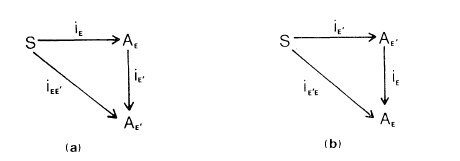
\includegraphics[width=0.7\textwidth]{imagenes/figura1.8.png}
    \caption*{Fig. 1.8. La acción selectiva de \( E \) seguida de \( E' \) (diagrama (a)) difiere de la acción selectiva resultante en el orden inverso (diagrama (b)).}
\end{figure}

%---------------------------------------------------------------------------------------------------------------------------------------------
%PAG 33
\newpage
\fancyhf{}
\fancyhead[r]{\thepage}
\begin{center}
{\fontsize{13}{16}\selectfont \textbf{SISTEMA}}
\end{center}
\vspace{0.5cm}

{\fontsize{13}{15}\selectfont
... sembrado a partir de unidades suministradas por el entorno: este último proporciona la oportunidad para el autoensamblaje, y por tanto para la emergencia. En resumen, el entorno de cualquier sistema es creativo —solo que es selectivo y excluyente más que permisivo.

\subsection*{3.4. Evolución}

El autoensamblaje puede resultar en evolución —y esto a nivel molecular, organísmico, poblacional y otros. 
Examinemos entonces el concepto general de evolución. Para ello comencemos por dilucidar el concepto general de descendencia: \\

\textbf{DEFINICIÓN 1.16} Sea \( S \) una colección de sistemas de algún tipo. Entonces para cualquier \( x \) y \( y \) en \( S \),

(i) \( x \) es un \textbf{antepasado inmediato} de \( y \) (o \( y \) \textbf{desciende inmediatamente} de \( x \)) si y solo si \( x \) y \( y \) pertenecen a la misma especie y \( x \) o una parte de \( x \) es un precursor en el ensamblaje de \( y \);

(ii) \( x \) es un \textbf{antepasado mediato} de \( y \) (o \( y \) \textbf{desciende mediatamente} de \( x \)) si y solo si existe un \( z \) en \( S \) tal que \( x \) es un antepasado inmediato de \( z \), y \( z \) un antepasado inmediato de \( y \);

(iii) \( x \) es un \textbf{antepasado} de \( y \) (o \( y \) \textbf{desciende} de \( x \)) si y solo si \( x \) es un antepasado inmediato o mediato de \( y \). Símbolo: \( x < y \);

(iv) la \textbf{ascendencia} de \( x \) es la colección de antepasados de \( x \):

\[A(x) = \{y \in S \mid y < x\};\]

(v) la \textbf{progenie} de \( x \) es la colección de cosas de las que \( x \) es antepasado:

\[P(x) = \{y \in S \mid x < y\};\]

(vi) el \textbf{linaje} de \( x \) es la unión de la ascendencia y la progenie de \( x \):

\[L(x) = \{y \in S \mid y < x \text{ o } x < y\}.\]

Claramente, la relación de ascendencia \( < \) es un orden parcial estricto. El grafo de \( < \) es entonces dirigido con aristas simples y sin bucles.

\textbf{Ejemplo 1} Los hidrocarburos descienden de \( C \) y \( H \), los polímeros de los respectivos monómeros, los ribosomas de moléculas de ARN y proteínas, los animales de sus padres, etc. \textbf{Ejemplo 2} La progenie de una bacteria que se reproduce por división binaria se ve así:
}

%---------------------------------------------------------------------------------------------------------------------------------------------
%PAG 34
\newpage
\fancyhf{}
\fancyhead[l]{\thepage}
\begin{center}
{\fontsize{13}{16}\selectfont \textbf{CAPÍTULO I}}
\end{center}
\vspace{0.5cm}

\begin{figure}[h!]
    \begin{minipage}{0.5\textwidth}
        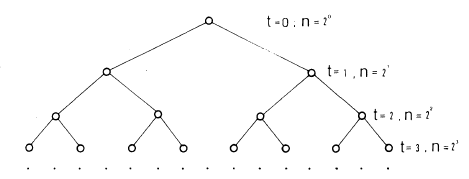
\includegraphics[width=\linewidth]{imagenes/pag.34.png}
    \end{minipage}%
    \hfill
    \begin{minipage}{0.4\textwidth}
        \raggedleft
        \fontsize{13}{15}\selectfont
        $t = 0, n = 2^0$ \\[1em]
        $t = 1, n = 2^1$ \\[1em]
        $t = 2, n = 2^2$ \\[1em]
        $t = 3, n = 2^3$
    \end{minipage}
\end{figure}

Si bien en muchos casos los miembros del linaje de un sistema pertenecen a la misma especie, a veces no es así. Cuando no lo hacen, el linaje constituye una línea evolutiva. Más precisamente, establecemos \\

\textbf{DEFINICIÓN 1.17} Sea \( L(x) \) el linaje de un sistema \( x \) de tipo \( K \). Entonces \( L(x) \) es un \textbf{linaje evolutivo} si y solo si al menos un antepasado o un descendiente de \( x \) pertenece a un tipo \( K' \) diferente de \( K \).
Las nociones de descendencia, linaje y linaje evolutivo se extienden a colecciones de sistemas:\\

\textbf{DEFINICIÓN 1.18} Sea \( S \) una familia de colecciones de sistemas: \( S = \{S_i \text{ es una colección de sistemas } \mid 1 \leq i \leq n\} \). Entonces para todos \( S_j \) y \( S_k \) en \( S \),

(i) \( S_k \) \textbf{desciende} de \( S_j \) si y solo si todo miembro de \( S_k \) desciende de algunos miembros de \( S_j \): \( S_j < S_k \);
(ii) el \textbf{linaje} de \( S_j \) es la familia de colecciones que descienden de \( S_j \) o de las cuales \( S_j \) desciende:

\[A(S_j) = \{X \in S \mid X < S_j \text{ o } S_j < X\};\]

(iii) \( A(S_j) \) es un \textbf{linaje evolutivo} si y solo si al menos uno de los antepasados o los descendientes de \( S \) está incluido en una especie diferente de la que incluye a \( S_j \).
Recordemos ahora que, según el Postulado 1.4, todo sistema se forma por ensamblaje. Dado que un sistema y sus precursores pertenecen a especies diferentes, se sigue que el ensamblaje resulta en especiación, es decir, la formación de nuevas especies. 
En otras palabras, tenemos\\

\textbf{TEOREMA 1.3} Todo sistema concreto pertenece a algún linaje evolutivo.

Para cerrar esta subsección, enfaticemos que las hipótesis precedentes se asumen válidas para sistemas de todo tipo —físicos, químicos, biológi-
}

%---------------------------------------------------------------------------------------------------------------------------------------------
%PAG 35
\newpage
\fancyhf{}
\fancyhead[r]{\thepage}
\begin{center}
{\fontsize{13}{16}\selectfont \textbf{SISTEMA}}
\end{center}
\vspace{0.5cm}

{\fontsize{13}{15}\selectfont
... cos, o sociales. Las peculiaridades de los sistemas de estos géneros de sistemas se estudiarán en capítulos sucesivos.

\vspace{0.5cm}
\begin{center}
{\fontsize{13}{16}\selectfont \textbf{4. SISTEMICIDAD}}
\end{center}
\vspace{0.5cm}

\subsection*{4.1. Integración, Cohesión, Coordinación}

Todo lo que es un sistema es también un todo, pero no a la inversa: un agregado de componentes independientes es un todo pero no uno integrado o unitario. (Compárese un ser vivo con sus cenizas.) Ahora bien, la sistematicidad o integración viene en grados: algunos sistemas están más estrechamente unidos que otros. El grado de integración depende de las conexiones o enlaces entre los componentes de un sistema en relación con las acciones desintegradoras del entorno. Si los acoplamientos internos son "positivos" (o "atractivos") y fuertes, el grado de integración es alto; si los enlaces son aún positivos pero débiles, el grado de integración es bajo; y si los enlaces son "negativos" (o "repulsivos"), no hay sistematicidad o integración en absoluto. Finalmente, si algunos de los enlaces son "positivos" mientras que otros son "negativos", el grado de integración depende de cuáles de ellos predominen. Por ejemplo, un núcleo atómico estable se mantiene unido por fuerzas nucleares que superan las repulsiones eléctricas; y una comunidad humana estable se mantiene unida por la participación en empresas de interés común, cuyo valor es mayor que el de la rivalidad o la competencia —hasta que, por supuesto, esta última se impone.

En el caso de los sistemas físicos, químicos y quizás también biológicos, lo que mide su grado de integración es su energía de enlace o, lo que es lo mismo, su energía de disociación. Esta es la energía mínima requerida para disociar el sistema en sus componentes. Es cero para un agregado. Pero tal medida no es universal: no se aplica a sistemas donde los enlaces de información juegan un papel integrador al menos tan importante como las fuerzas propiamente dichas —como es el caso de los sistemas sociales. En resumen, no existe una medida universal del grado de integración o cohesión de un sistema. Sin embargo, podemos asumir el postulado metodológico de que se puede establecer una medida para cada género de sistema, o incluso para cada clase de modelos, independientemente de la naturaleza de los componentes de los sistemas representados por tales modelos.

\textbf{Ejemplo} Dos cosas, etiquetadas 1 y 2, forman un sistema lineal si los componentes de la función de estado \( F = \langle F_1, F_2 \rangle \) de este último satisfacen las ecuaciones de tasa
\[\dot{F}_1 = a_{11}F_1 + a_{12}F_2, \quad \dot{F}_2 = a_{21}F_1 + a_{22}F_2,\]
}

%---------------------------------------------------------------------------------------------------------------------------------------------
% PAG 36
\newpage
\fancyhf{}
\fancyhead[l]{\thepage}
\begin{center}
{\fontsize{13}{16}\selectfont \textbf{CAPÍTULO I}}
\end{center}
\vspace{0.5cm}

{\fontsize{13}{15}\selectfont
donde los \( a_{ij} \) son en general números complejos. El grado de integración o cohesión del sistema puede entonces definirse como
\[w = \frac{|a_{12}|}{|a_{11} + a_{12}|} + \frac{|a_{21}|}{|a_{21} + a_{22}|}.\]
Si los \( a_{ij} \) no son constantes sino dependientes del tiempo, \( w \) mismo dependerá del tiempo. En general, \( w: T \rightarrow [0, 1] \).
Si \( a_{12} = a_{21} = 0 \), los componentes no forman un sistema; en cualquier otro caso sí lo hacen. En particular, si el componente 1 controla el componente 2, entonces \( a_{12} = 0 \) y \( a_{21} \neq 0 \), de donde \( 0 < w \leq 1 \). Y si hay interacción simétrica, \( a_{12} = a_{21} \neq 0 \). Finalmente, si todos los \( a_{ij} \) son iguales a la unidad, \( w = 1 \), es decir, el sistema es maximalmente cohesivo.

Asumamos entonces que es posible definir en cada caso una medida \( w: T \rightarrow [0, 1] \) del grado de integración de sistemas de cualquier tipo dado. Entonces, 
trazando el curso de los valores de \( w \) podemos seguir la historia del sistema desde su construcción hasta su descomposición a través de su etapa estable, si la hay. En otras palabras, podemos introducir. \\

\textbf{DEFINICIÓN 1.19} Sea \( \sigma \) un sistema con grado de cohesión o integración \( w(t) \) en el tiempo \( t \). Entonces \( \sigma \) es \textit{estable} durante el intervalo de tiempo \( \tau \) si y solo si \( w(t) \) es constante para todo \( t \in \tau \) o a lo sumo fluctúa dentro de límites alrededor de un valor constante. De lo contrario \( \sigma \) es \textit{inestable} y, en particular,
(i) se \textit{construye} (integra o ensambla) si y solo si su grado de integración aumenta en el tiempo;
(ii) se \textit{descompone} (desintegra o desmantela) si y solo si su grado de integración disminuye en el tiempo.

El grado de integración o cohesión de un sistema está relacionado con su tamaño o número de componentes, así como con la naturaleza de estos últimos. 
Un sistema con un número extremadamente grande de componentes puede ser inestable y finalmente descomponerse en varios subsistemas: siempre hay algún límite superior para el tamaño de un sistema —un límite al crecimiento. Véase la Figura 1.9. 
Resumimos esta generalización empírica en\\

\textbf{POSTULADO 1.7} Para cada tipo de sistema hay un \textit{tamaño optimo}, es decir, un número de componentes que maximiza el grado de integración (cohesión) del sistema en el entorno dado. Ese número se llama el \textit{tamaño crítico}.
Una consecuencia inmediata de este supuesto es que, para cada tipo de sistema, hay (a) un \textit{tamaño umbral}, es decir, un número de componentes por debajo
}

%---------------------------------------------------------------------------------------------------------------------------------------------
% PAG 37
\newpage
\fancyhf{}
\fancyhead[r]{\thepage}
\begin{center}
{\fontsize{13}{16}\selectfont \textbf{SISTEMA}}
\end{center}
\vspace{0.5cm}

{\fontsize{13}{15}\selectfont
\begin{figure}[h!]
    \centering
    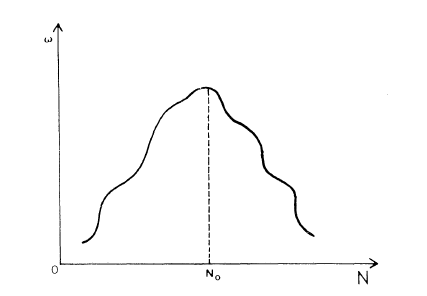
\includegraphics[width=0.7\textwidth]{imagenes/figura1.9.png}
    \caption*{Fig. 1.9. Grado de integración (cohesión) por número de componentes vs. número total de componentes. \( N_0 \) = tamaño óptimo o crítico.}
\end{figure}
del cual el agregado no forma un sistema, y (b) un \textit{tamaño máximo}, i.e. a es decir, un número por encima del cual el sistema se descompone.
\textbf{Observación 1} A diferencia de la mayoría de los otros axiomas de nuestra teoría, el Postulado 1.7 es empíricamente comprobable. 
Por una parte, bien podría ser que para sistemas de ciertos tipos haya más de un solo tamaño crítico. Si este fuera el caso, tendríamos que hacer un pequeño ajuste en el Postulado 1.7.
 \textbf{Observación 2} La acreción por atracción gravitacional parecería refutar nuestro postulado. No lo hace, porque el mismo proceso aumenta la densidad de la materia y la energía de radiación, y esto eventualmente establece reacciones nucleares que pueden conducir a la explosión o al colapso. \par
El axioma precedente concierne a la integridad general o cohesión de un sistema sin tener en cuenta la integración de sus subsistemas. 
Si un sistema tiene subsistemas, no solo componentes, entonces la cohesión de los subsistemas compite con la del sistema general. \textbf{Ejemplo 1} Una molécula con todas sus valencias saturadas es estable, por lo que cohíbe pobremente con moléculas similares, por ejemplo, sus compañeros componentes en un polímero. 
En general, cuanto mayor es la complejidad de una molécula, menor es su energía de enlace general. \textbf{Ejemplo 2} Una familia humana grande tiene interacciones más débiles con el resto de la sociedad, por miembro familiar, que una familia pequeña: los miembros de una familia grande gastan una mayor cantidad de energía interactuando entre ellos que con su entorno social. 
Por lo tanto, aunque les va bien en casos de desastre, pueden no ser buenos ciudadanos.
Comprimimos estas observaciones en
}

%---------------------------------------------------------------------------------------------------------------------------------------------
%PAG 38
\newpage
\fancyhf{}
\fancyhead[l]{\thepage}
\begin{center}
{\fontsize{13}{16}\selectfont \textbf{CAPÍTULO I}}
\end{center}
\vspace{0.5cm}

{\fontsize{13}{15}\selectfont
\textbf{POSTULADO 1.8} Cuanto más cohesivo es cada subsistema, menos cohesivo es el sistema total.

Un problema para el diseñador de sistemas, ya sea un ingeniero o un científico social aplicado, es dar con una estructura que maximice la integridad general. No puede maximizar la cohesión de cada subsistema porque entonces este se vuelve autosuficiente en lugar de servir al todo. 
Y no puede minimizar las integridades parciales porque entonces los subsistemas se volverían inestables (poco confiables). Una solución de compromiso es elegir subsistemas de cohesión media y hacer que más de uno realice una función o rol dado. Tal diseño mejora la confiabilidad del sistema independientemente de su naturaleza. Véase la Figura 1.10.
Finalmente, otro concepto relevante para el de sistematicidad es la noción de \textbf{coordinación}, que debe distinguirse del de integración. Si la integración falla, el sistema sufre una descomposición estructural. 
Por otro lado, la coordinación concierne a la relación entre componentes o funciones que resulta en el mantenimiento funcional. Si la coordinación falla, el sistema sufre una descomposición funcional. Puede haber integración sin coordinación, pero no a la inversa. 
Una máquina compleja desajustada está integrada pero no coordinada. Por otro lado, los organismos están coordinados y \textit{a fortiori} integrados mientras viven. Una posible caracterización del concepto de coordinación viene dada por\\

\textbf{DEFINICIÓN 1.20} Si \( x \) e \( y \) están en la composición o en la estructura de un sistema, entonces se dice que \( x \) e \( y \) están \textbf{coordinados} si y solo si contribuyen conjuntamente a la integridad del sistema.

La coordinación no excluye la inhibición. Todo lo contrario: cuando
}

\begin{figure}[h!]
    \centering
    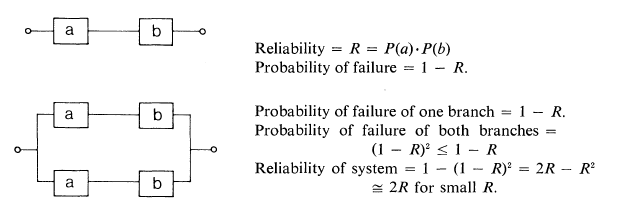
\includegraphics[width=0.7\textwidth]{imagenes/figura1.10.png}
    \caption*{Fig. 1.10. Aumento de la confiabilidad general (o grado de integración), aumentando la redundancia, es decir, el número de subsistemas que realizan la misma función. \( P(a) \) es la probabilidad de que el componente \( a \) realice su(s) función(es) regular(es).}
\end{figure}

%---------------------------------------------------------------------------------------------------------------------------------------------
%PAG 39
\newpage
\fancyhf{}
\fancyhead[r]{\thepage}
\begin{center}
{\fontsize{13}{16}\selectfont \textbf{SISTEMA}}
\end{center}
\vspace{0.5cm}

{\fontsize{13}{15}\selectfont
La coordinación es resultado del control incluye retroalimentación, que, cuando es negativa, es un tipo de inhibición. De hecho, sin tal control, la excitación podría destruir el sistema. 
Pero, por supuesto, puede haber coordinación sin la intervención de un sistema de control. Por ejemplo, el cuerpo calloso une los dos hemisferios cerebrales en los vertebrados y así hace posible su coordinación, pero no es un sistema de control en sí mismo. 
Por otro lado, todo el sistema nervioso central, que es un controlador, coordina todos los subsistemas que componen el organismo vertebrado.

Hasta aquí el concepto de totalidad. Ahora nos volvemos hacia las tres principales doctrinas filosóficas concernientes a los todos.

\subsection* {4.2. Holismo, Atomismo, Sistemismo}

Hay tres doctrinas posibles concernientes a los todos: holismo, atomismo y sistemismo. El holismo es la visión ontológica que enfatiza la integridad de los sistemas a expensas de sus componentes y las acciones mutuas entre ellos. 
Se caracteriza por las siguientes tesis.

H1 El todo precede a sus partes. A primera vista, esta tesis parece verdadera. Así, antes de ir a cortarse el pelo debemos haber crecido algo de pelo. 
Pero, por supuesto, el pelo creció gradualmente, no de repente: se convirtió en un todo en el curso de un proceso de multiplicación de partes (células). Antes de hacer una declaración general sobre qué precede a qué, deberíamos examinar el proceso real en cuestión. 
Un sistema precede a sus componentes solo durante un proceso de descomposición; les sucede durante el proceso de síntesis o formación. En cualquier caso, la existencia de un sistema puede no ser obvia: puede requerir una explicación en términos tanto de las acciones mutuas de las partes como del entorno. No se buscará tal explicación si el todo se da por sentado y se considera como la base última para la existencia de sus partes.

H2 El todo actúa sobre sus partes. Por ejemplo, se dirá que las necesidades del organismo (o la sociedad) como un todo dictan el funcionamiento de sus partes. 
Pero, por supuesto, no habría todo si no fuera por la coordinación de sus partes. No hay acción del todo sobre sus partes; más bien, hay acciones de algunos componentes sobre otros. 
Así, los modos de vibración de cualquier partícula individual en un cuerpo elástico están influenciados por el movimiento de las otras partículas; igualmente, el comportamiento de cualquier persona está parcialmente determinado por el de sus compañeros miembros de la sociedad. 
En todos estos casos no tenemos el todo actuando sobre sus partes, sino que algunos o incluso todos los componentes restantes del sistema actúan sobre el componente dado,
}

%---------------------------------------------------------------------------------------------------------------------------------------------
%PAG 40
\newpage
\fancyhf{}
\fancyhead[l]{\thepage}
\begin{center}
{\fontsize{13}{16}\selectfont \textbf{CAPÍTULO I}}
\end{center}
\vspace{0.5cm}

{\fontsize{13}{15}\selectfont
o el comportamiento de este último está parcialmente determinado por el lugar que ocupa en el sistema, en particular por su función o rol.

H3 \textit{El todo es más que la suma de sus partes}. Tal como está, la tesis es apenas inteligible. Se vuelve inteligible si por 'suma' uno significa la yuxtaposición (suma física o asociación +) que encontramos en la Sec. 1.6, y si por 'más' uno significa que el todo, siempre que sea un sistema, 
tiene propiedades emergentes que sus componentes carecen (cf. Sec. 3.2). Reformulada de esta manera, es decir, de una manera no holística, H3 adquiere un sentido definido —pero resulta ser solo parcialmente verdadera. De hecho, aunque todo sistema es un todo, no toda totalidad es un sistema; así, 
la mera agregación de cosas no necesita resultar en un todo integrado o sistema (cf. Sec. 4.1.). Lo que hace que un todo sea un sistema son precisamente las acciones ejercidas por algunas de sus partes sobre otras. Pero al holista no le importa la revelación de tales acoplamientos, es decir, la estructura del sistema: desprecia el análisis.

H4 \textit{Los todos emergen bajo la acción de agentes que trascienden tanto las acciones entre los componentes como las influencias ambientales}. 
Por ejemplo, la morfogénesis está guiada por una entelequia, o \textit{élan vital}, o campo morfogenético externo a los componentes. 
En resumen, la formación de totalidades trasciende sus componentes y es rastreable a entidades inescrutables. Hasta aquí la cuenta holística de la formación de los todos. Huelga decir que la ciencia no tiene uso para tales principios de organización secretos y, por lo tanto, incontrolables. 
En cambio, la ciencia actúa sobre un principio de inmanencia, no de trascendencia, a saber, este: Solo los componentes, la forma en que se unen y el entorno determinan qué tipo de cosa será una totalidad. (De ahí nuestra representación de un sistema por la terna ordenada: composición-entorno-estructura.)

H5 \textit{Las totalidades no pueden ser explicadas por el análisis: son irracionales}. Esta tesis es trivialmente verdadera si por 'análisis' se entiende solo descomposición en partes, ya que entonces solo se revela la composición de un sistema pero no su estructura. 
Si esta última se deja fuera, entonces, por supuesto, se vuelve imposible dar cuenta de las propiedades sistémicas o gestálticas de una totalidad. Pero el físico no afirma que el agua es solo un agregado de moléculas de \( H_2O \), y el sociólogo no afirma que la sociedad es solo una colección de personas. 
En cualquier caso, los enlaces entre los componentes (enlaces de hidrógeno, relaciones de trabajo, o lo que sea) deben ser revelados o hipotetizados para entender la formación, cohesión y eventual descomposición de una totalidad. Tal análisis es la base conceptual para cualquier síntesis efectiva o construcción ascendente, así como para el análisis efectivo o desintegración de un sistema.

H6 \textit{El todo es mejor que cualquiera de sus partes}. Este juicio de valor tiene
}